The \emph{Events} page contains a grid with all events that our association organizes.  By clicking on each event image or name it is possible to navigate to the event's details page. Through the group links into the left side menu is possible to filter events depending on their type and date (the date filter is different from "Events by Month x" multiple group).

\begin{figure}[h!]
		\centering
		\begin{minipage}[b]{1\textwidth}
    			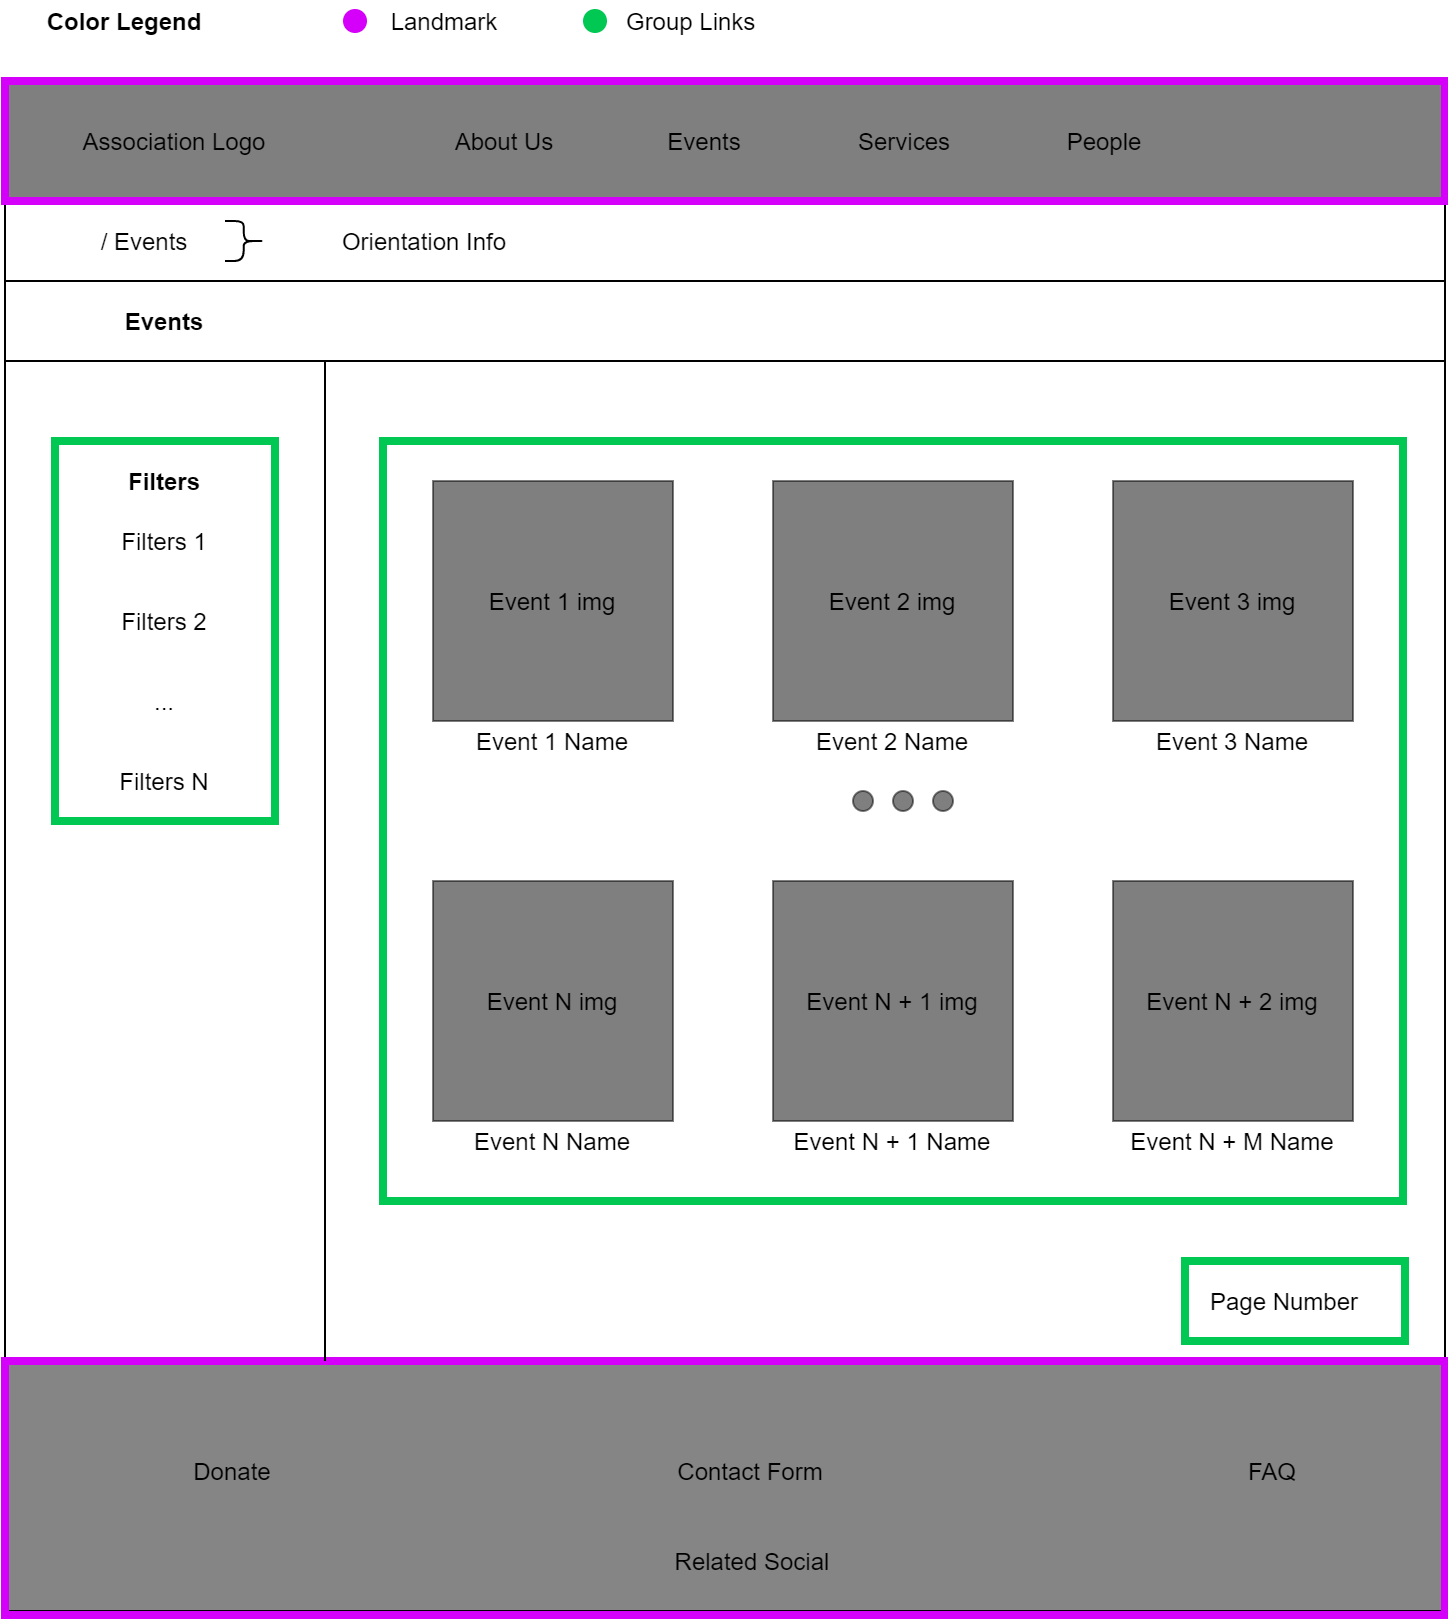
\includegraphics[width=\textwidth]{./assets/events.png}
			\caption{Events Page - Design in the small}
		\end{minipage}
	\end{figure}
\FloatBarrier 
\vspace{1cm}
\hspace{-1cm}
Events' details can be found in Event page, which contains:
\begin{itemize}
	\item all event's information stored into the database such as the promotion image, practical info (like event date and location),  			a brief description, etc. etc.
	\item the transition links to all services that the association provide during the selected event
	\item the transition link to the volunteers' details that are the point of reference and organizers of the selected event
\end{itemize} 

\begin{figure}[h!]
		\centering
		\begin{minipage}[b]{1\textwidth}
    			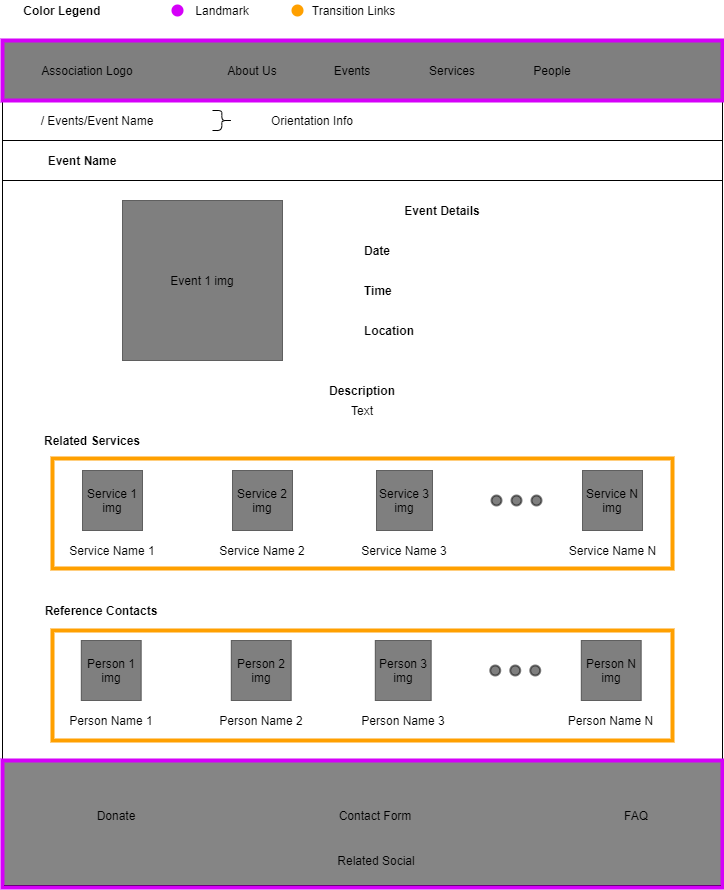
\includegraphics[width=\textwidth]{./assets/eventdetails.png}
			\caption{Event Page - Design in the small}
		\end{minipage}
\end{figure}
\FloatBarrier
